Teniendo en una mano el \textit{CMM} y en la otra el \textit{Winning-Percentage}, uno estar\'ia tentado a atinar una respuesta a la pregunta "¿C\'omo se comparan?". En esta secci\'on vamos a presentar resultados a partir de los cu\'ales se puedan observar diferencias o similitudes.

Veamos qu\'e ocurre cuando ponemos a prueba ambos m\'etodos en la NBA con la condicion de que todos los equipos disputaron \textit{aproximadamente} 41 encuentros, que es la mitad de una temporada regular. Los resultados que obtuvimos fueron los siguientes: \\

\begin{figure}[h!]
  \begin{center}
	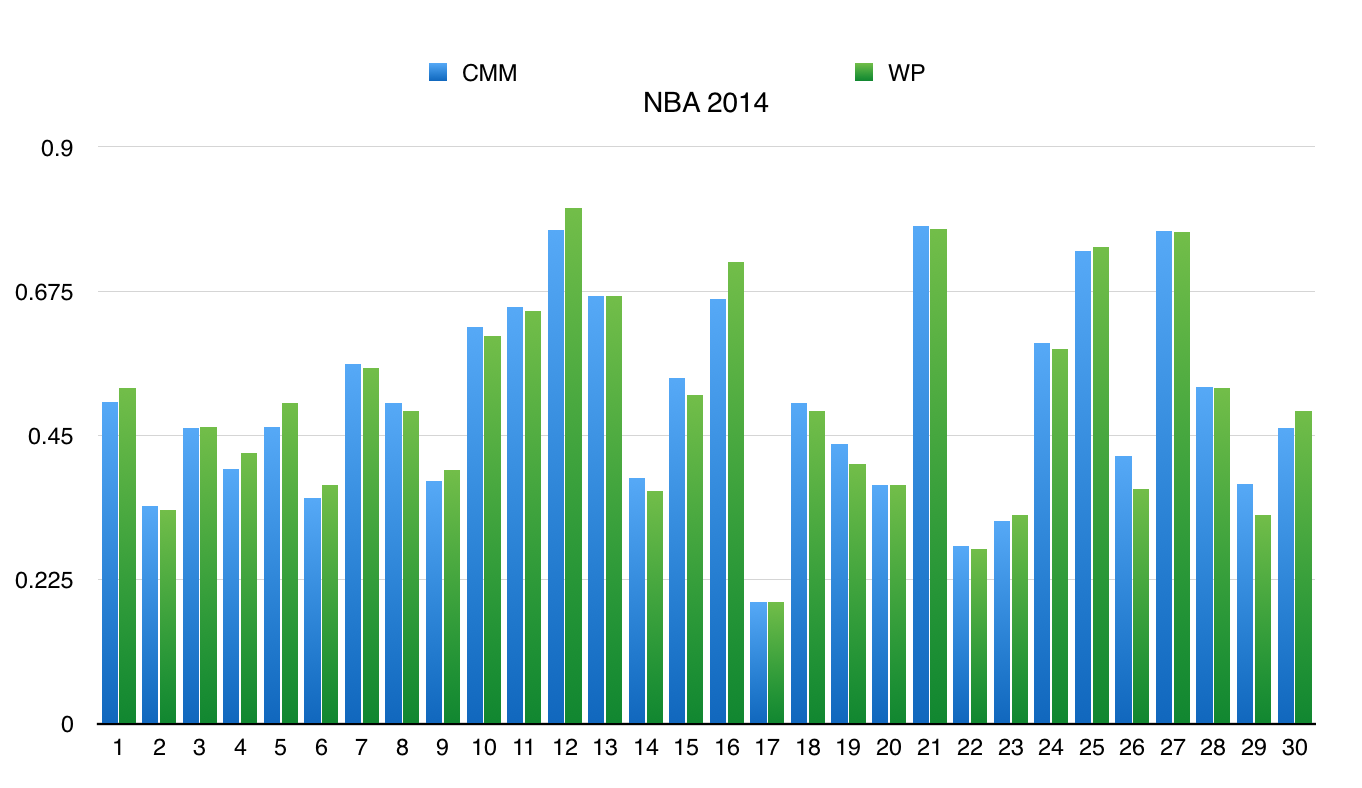
\includegraphics[scale=0.50]{imagenes/cualitative/comparative/nba2014.png}
	\caption{Season 2014}
%	\label{bChange}
  \end{center}
\end{figure}

\begin{figure}[h!]
  \begin{center}
	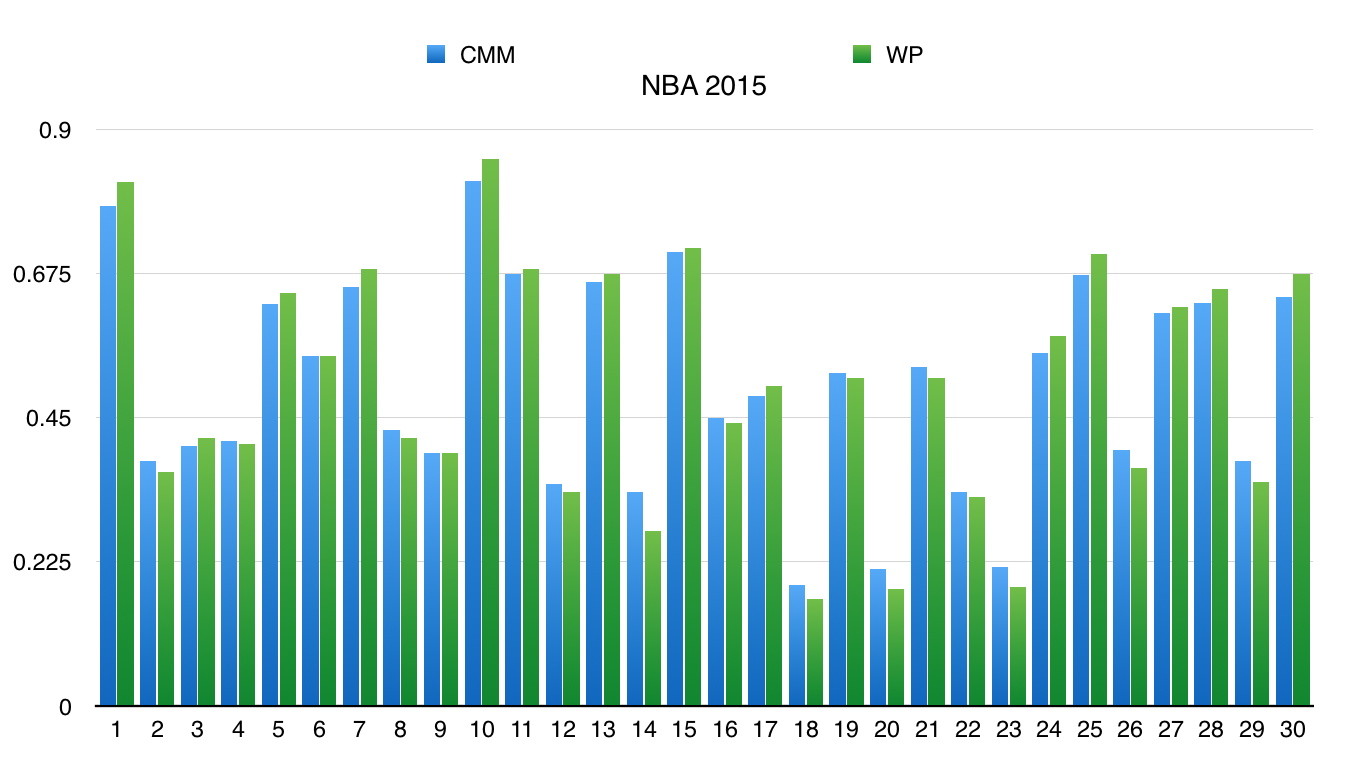
\includegraphics[scale=0.50]{imagenes/cualitative/comparative/nba2015.png}
	\caption{Season 2015}
%	\label{bChange}
  \end{center}
\end{figure}

\begin{figure}[h!]
  \begin{center}
	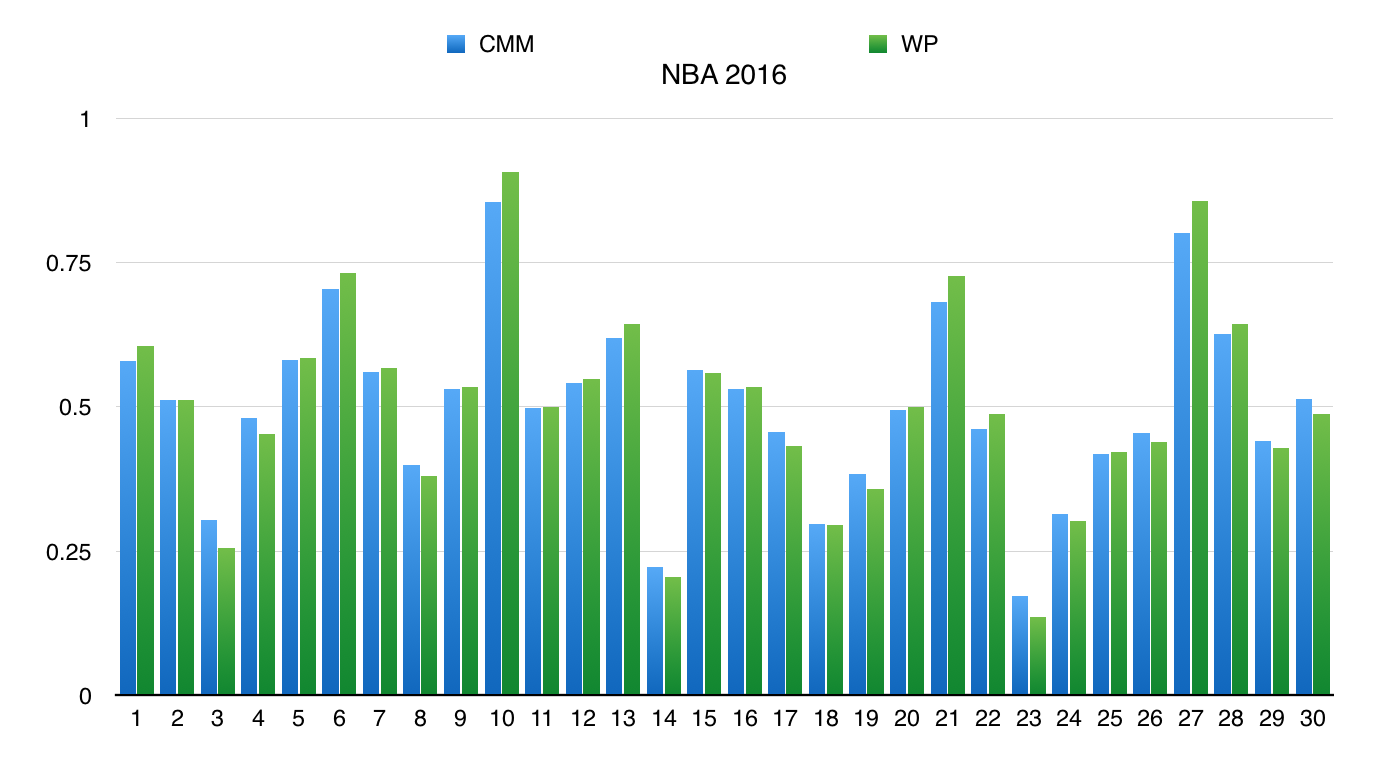
\includegraphics[scale=0.50]{imagenes/cualitative/comparative/nba2016.png}
	\caption{Season 2016}
%	\label{bChange}
  \end{center}
\end{figure}

Se puede observar claramente que no hay diferencias sustanciales y esto tiene que ver con que observamos un caso \textit{"promedio"}. Una explicaci\'on m\'as matem\'atica yace en lo planteado en \textbf{[1]}, en el estimador de $r_{i}$, obtenido a partir de la \textbf{Regla de sucesi\'on de Laplace [2]}. Ocurre que $r_{i} = \frac{1 + w_{i}}{2 + n_{i}} \approx \frac{w_{i}}{n_{i}} \approx \frac{w_{i}}{k}$ donde este \'ultimo termino es el valor exacto que se obtiene de plantear el \textit{Winning-Percentage} sobre el equipo $i$, para este escenario. 

Al ser un estimador, y tener similitudes con el mismo, tiene sentido que, siendo un caso aleatorio, a valores m\'as grandes tiendan a parecerse.

Pero esto ocurre en un caso real, y la realidad tiende a comportarse parecido al promedio. Contrastemos esto con casos particulares. \\

\textbf{Hipotesis}: partidos ganados / partidos jugados, no tiene en cuenta la infomaci\'on sobre contra a qui\'en les toc\'o jugar.

Para este experimento, lo plantedo fue un conjunto de participantes $\Gamma = \{1,2,...,5\}$, donde se pone al equipo $1$ en la siguiente situaci\'on:

El equipo $1$ en 4 ocasiones vence al equipo $2$, 3 al equipo $3$, 2 al equipo $4$ y, finalmente, 1 al contricante $5$ y los resultados fueron: \\

\begin{figure}[h!]
  \begin{center}
	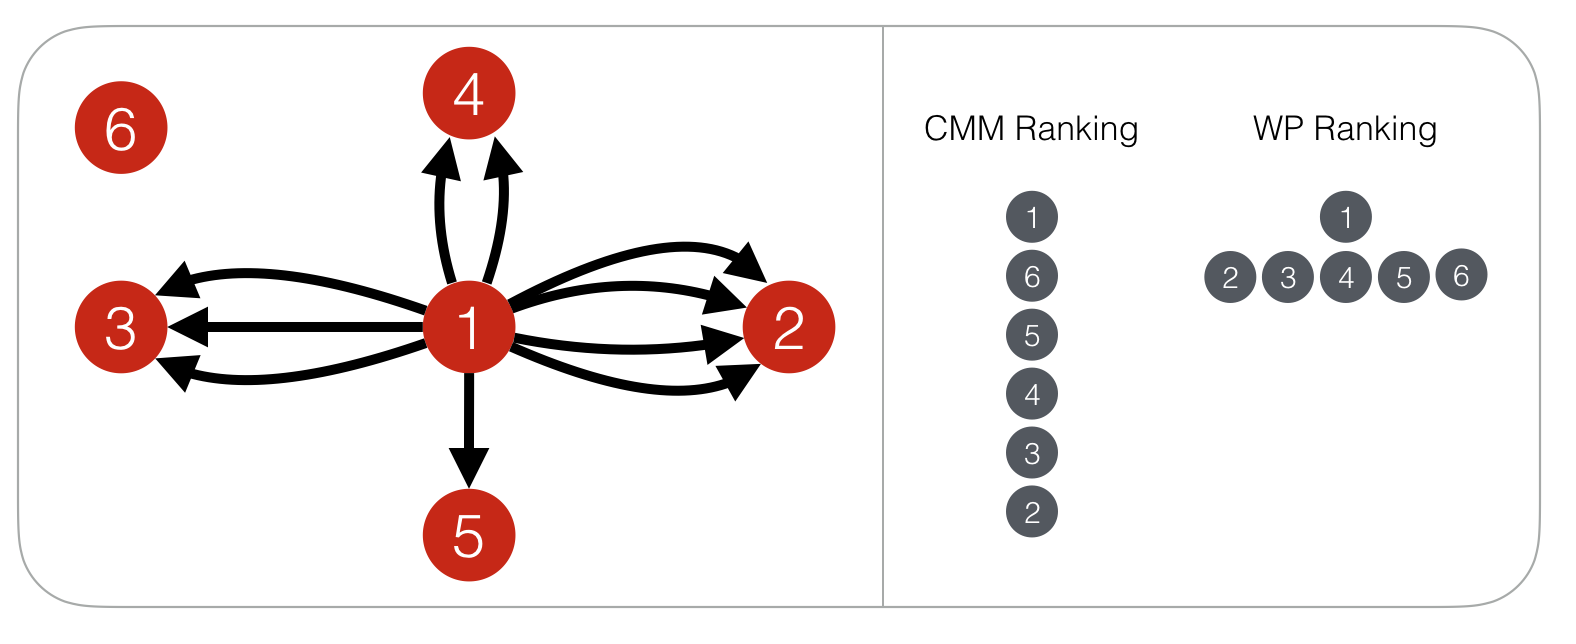
\includegraphics[scale=0.50]{imagenes/cualitative/comparative/comparative2.png}
	\caption{Experimento}
%	\label{bChange}
  \end{center}
\end{figure}

Para ambos casos, el algoritmo WP asigna $r_1 = 1$ y $r_i = 0, i = 2, ..., 6$. \footnote{Esto refuerza el hecho de haber usado \textbf{[2]} en el CMM: El resto de los equipos tiene el mismo rating habiendo perdido (además de jugado) distinta cantidad de encuentros.} En cuanto a ratings respecta, el equipo $2$ es efectivamente el \'ultimo y por ende ocurre lo observado. \\

\textbf{Hipotesis}: El m\'etodo CMM previene ``sobre-calificar'' a un equipo venciendo reiteradamente a un equipo con bajo ranking, en contraposici\'on al WP. En otras palabras, esto quiere decir que no deber\'ia implicar el mismo aumento de rating vencer a un participante con rating elevado que a uno con rating bajo. \\

La configuraci\'on del schedule que buscamos para ejemplificar nuestra hipotesis fue uno tal que tenemos $\Gamma = \{1,2,...,4\}$ en el cual los equipos $1$, ..., $3$ juegan entre s\'i y, por ende, podemos armar un rating \textit{parcial} entre ellos. Luego, hacemos jugar al parcialmente ``peor'' participante, entre los mismos, contra el equipo $4$ de tal forma que ambos algoritmos generan casos distintos. Esta fue la configuraci\'on: \\

Y el resultado fue: \\

\begin{figure}[h!]
  \begin{center}
	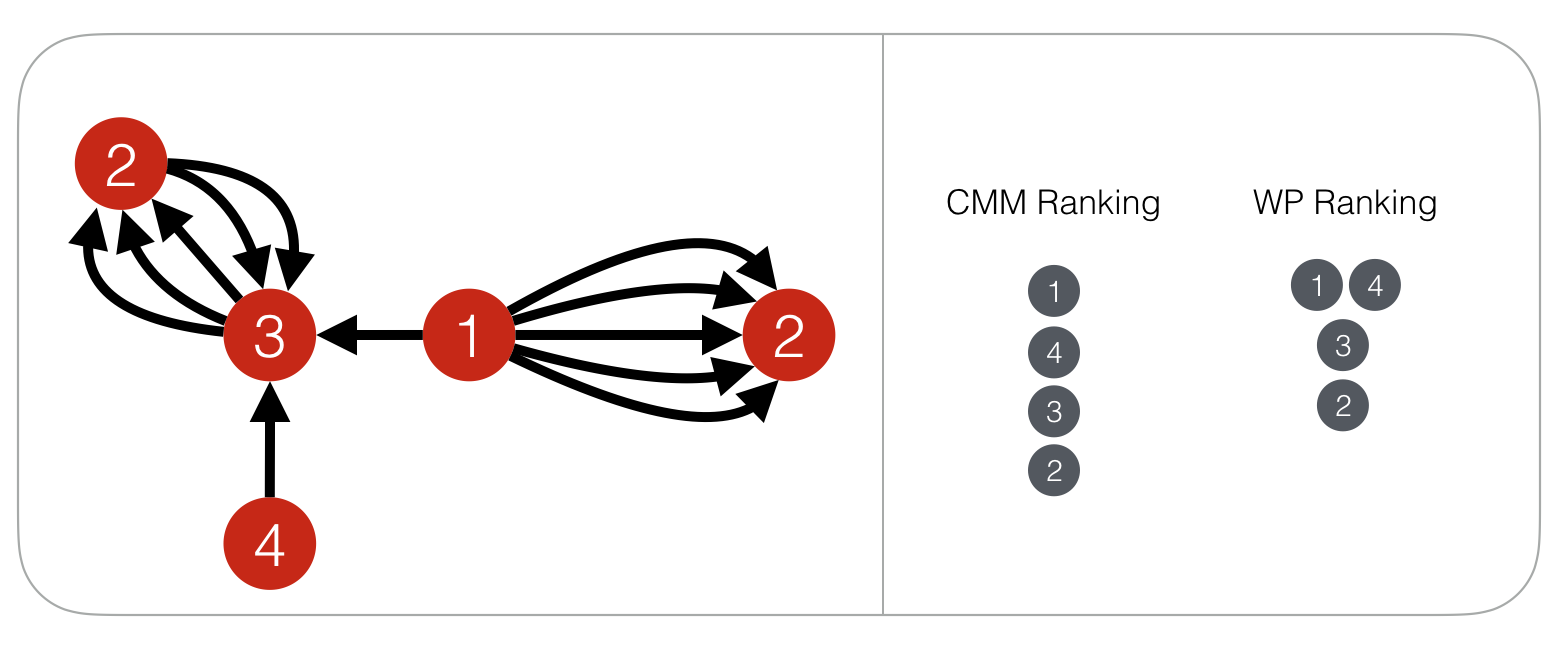
\includegraphics[scale=0.50]{imagenes/cualitative/comparative/comparative3.png}
	\caption{Experimento}
%	\label{bChange}
  \end{center}
\end{figure}


La ``l\'ogica'' indica que ganarle al peor de un grupo no deber\'ia implicar un ascenso importante en los ratings, mucho menos ser mejor o igual que el primero, y en este caso comprobamos que el WP no siempre sigue esa l\'ogica.
